\chapter{Triangulácia}
\label{kap:triangulation}

Usporiadanú trojicu množín $(V, E, F)$, kde $V$ je množina vrcholov daná ich súradnicami, 
$E$ je množina neorientovaných hrán daná 
dvojicou vrcholov z $V$, $F$ je množina stien daných $n$-ticou vrcholov z $V$, kde $n \geq 3$, 
nazývame \textit{mesh}.

V prípade, že všetky steny sú dané trojicou vrcholov, nazývame tento mesh trianguláciou.

Trianguláciou implicitne definovanej plochy nazývame aproximáciu tejto plochy trojuholníkovým meshom.

Podľa článku \mbox{\textit{Adaptive implicit surface polygonization using marching triangles}~\cite{akkouche2001adaptive}},
vhodná triangulácia by mala spĺňať viacero podmienok. Vygenerovaný mesh by mal byť konzistentný, 
teda bez dier alebo rozpojených vrcholov, hrán alebo stien. Na \mbox{obrázku \ref{obr:torus_holes}}
môžeme vidieť ako vyzerá nekonzistentná triangulácia torusu, pričom na 
\mbox{obrázku \ref{obr:torus_no_holes}} sa nachádza vhodná triangulácia, bez dier. 

\begin{figure}
    \centerline{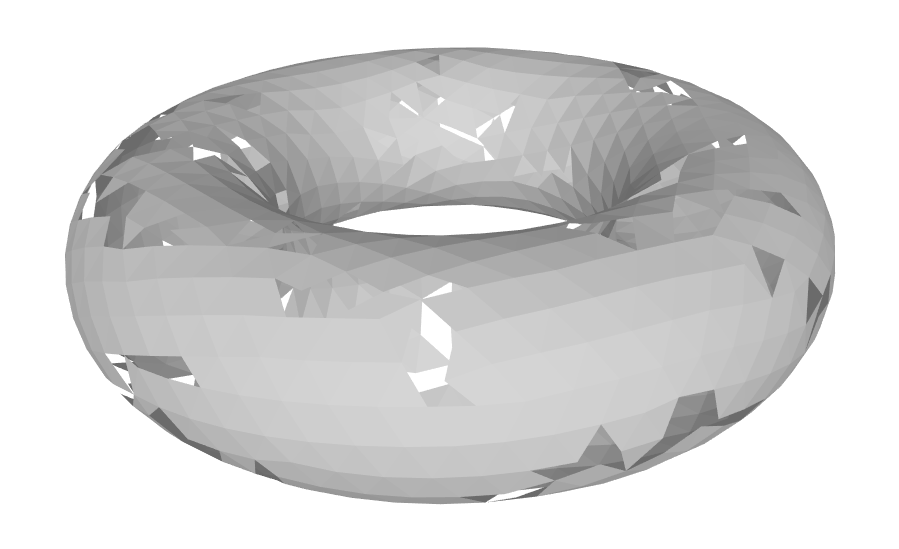
\includegraphics[width=0.8\textwidth]{images/torus_holes}}
    \caption[Príklad nekonzistentnej triangulácie]{Nekonzistentná triangulácia torusu s dierami.}
    %id obrazku, pomocou ktoreho sa budeme na obrazok odvolavat
    \label{obr:torus_holes}
\end{figure}

\begin{figure}
    \centerline{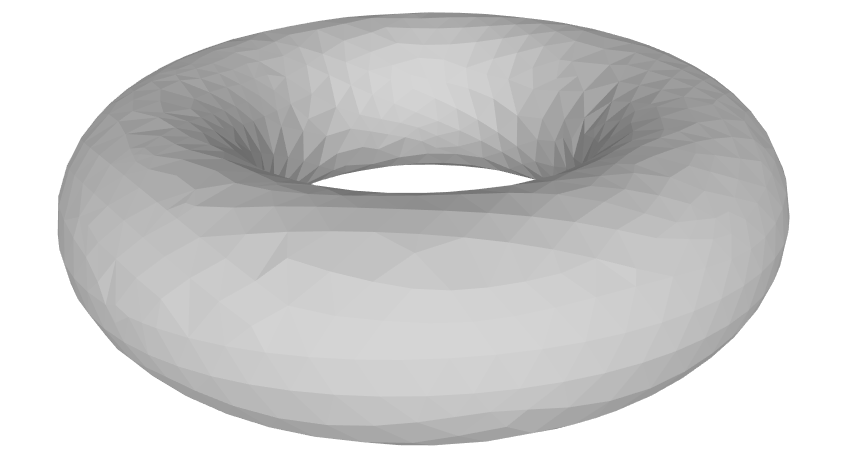
\includegraphics[width=0.8\textwidth]{images/torus_no_holes}}
    \caption[Príklad konzistentnej triangulácie]{Konzistentná triangulácia torusu bez dier.}
    %id obrazku, pomocou ktoreho sa budeme na obrazok odvolavat
    \label{obr:torus_no_holes}
\end{figure}

Ďalej by vzniknutá triangulácia mala byť topologicky homeomorfná 
so zadanou plochou. Aproximácia by mala byť dostatočne presná a trojuholníky by mali 
byť čo najpravidelnejšie. Naviac vhodná triangulácia plochy by sa mala prispôsobiť zakriveniu plochy,
teda mala by vyprodukovať menšie trojuholníky v miestach s väčším zakrivením, a naopak väčšie
trojuholníky v miestach s menším zakrivením, túto vlastnosť nazývame \textit{adaptivita na krivosť}~\cite{akkouche2001adaptive}.

Na trianguláciu implicitne definovanej plochy sa používa množstvo rôznych prístupov, 
avšak nie každá metóda dokáže vyprodukovať trianguláciu spĺňajúcu všetky kritéria, 
ktoré sme popísali. Na druhú stranu, presnejšie algoritmy, ktoré dokážu vyprodukovať 
kvalitné meshe potrebujú viac výpočtového času. 

K najrýchlejším metódam triangulácie implicitne definovanej plochy patria takzvané prístupy pomocou rozkladu
priestoru, ktoré delia priestor obsahujúci plochu na menšie bunky, napríklad kocky alebo štvorsteny. 
Následne pomocou znamienka funkcie definovanej implicitne vyhodnotenej vo vrcholoch týchto buniek
sa zistí, či sa vrcholy buniek nachádzajú pod povrchom alebo nad povrchom. 
Pomocou numerických metód sa vypočítajú približné priesečníky hrán týchto buniek s 
implicitnou funkciou a použijú sa vyhľadávacie tabuľky na zistenie triangulácie plochy v danej bunke. 
To, že tieto metódy patria k najrýchlejším nám napovedá, že nebudú príliš presné. Mnoho vedcov sa
však zameralo na tieto rýchle algoritmy a pomocou následného spracovania triangulácie sa im 
podarilo upraviť dané \textit{meshe} na kvalitnejšie. 
Medzi najznámejšie algoritmy rozkladajúce priestor
patrí algoritmus \textit{Marching Cubes}~\cite{lorensen1987marching} a \textit{Marching Tetrahedra}~\cite{doi1991efficient}. 
Na skvalitnenie algoritmu \textit{Marching Cubes} sa pozreli napríklad
autori Carlos A. Dietrich, et. al~\cite{dietrich2009marching}, 
ktorí sa zameriavajú na odstránenie úzkych a malých trojuholníkov
z výsledného \textit{meshu}.

Ku kvalitnejším, avšak pomalším prístupom patria takzvané prístupy sledovania plochy.
Tieto algoritmy sa začínajú v bode ležiacom na ploche (alebo dostatočne blízko plochy) a 
postupne sledujú plochu a vytvárajú polygóny. Tu sa vyskytuje jedna z nevýhod implicitne definovanej
plochy - nájsť bod ležiaci na ploche je ťažšie ako pri explicitnom vyjadrení. Medzi najznámejšie 
algoritmy sledujúce plochu patrí \textit{Marching Triangles}~\cite{hilton1996marching}.
Výstupom algoritmu môžu byť okrem samotného \textit{meshu} aj normály vo vrcholoch trojuholníkov triangulácie.
Tieto normály sa používajú najmä na čo najpresnejšie tieňovanie triangulácie.

\section{Marching Cubes}

Algoritmus \textit{Marching Cubes}~\cite{lorensen1987marching} patrí k najznámejším algoritmom používaným
na trianguláciu implicitne definovanej plochy. Prvý krát bol prezentovaný v roku 1987. Patrí k najrýchlejším
algoritmom avšak výsledok nespĺňa mnoho kritérií kvality triangulácie. 

Autori algoritmu sa rozhodli pre prístup spočívajúci v rozdelení zložitejšieho problému na 
jednoduchšie podproblémy, ktoré sa dajú ľahšie riešiť. Následne algoritmus 
spojí tieto riešenia do jedného.

Rozdelenie problému spočíva v podrozdelení priestoru, v ktorom sa nachádza zadaná plocha na kocky 
so zvolenou dĺžkou hrany. 
Následne sa pre každú kocku vypočíta, ktoré vrcholy sa nachádzajú pod povrchom (alebo na ňom) 
a ktoré nad povrchom. Keďže každá kocka má 8 vrcholov a každý vrchol môže nadobudnúť hodnotu $1$, ak sa 
nachádza pod povrchom alebo na ňom, alebo hodnotu $0$, ak sa nachádza nad povrchom, existuje práve 
$2^8 = 256$ možností. Vďaka symetriám sa však autorom podarilo znížiť tento počet len na 15 rôznych možností.
Pre tieto možnosti vytvorili tabuľku, kde pomocou 8 bitového binárneho čísla označujúceho charakteristiku
kocky vyhľadávali dané triangulácie. Zredukovanú vyhľadávaciu tabuľku môžeme vidieť na obrázku \ref{obr:lookup_table}.

\begin{figure}
    \centerline{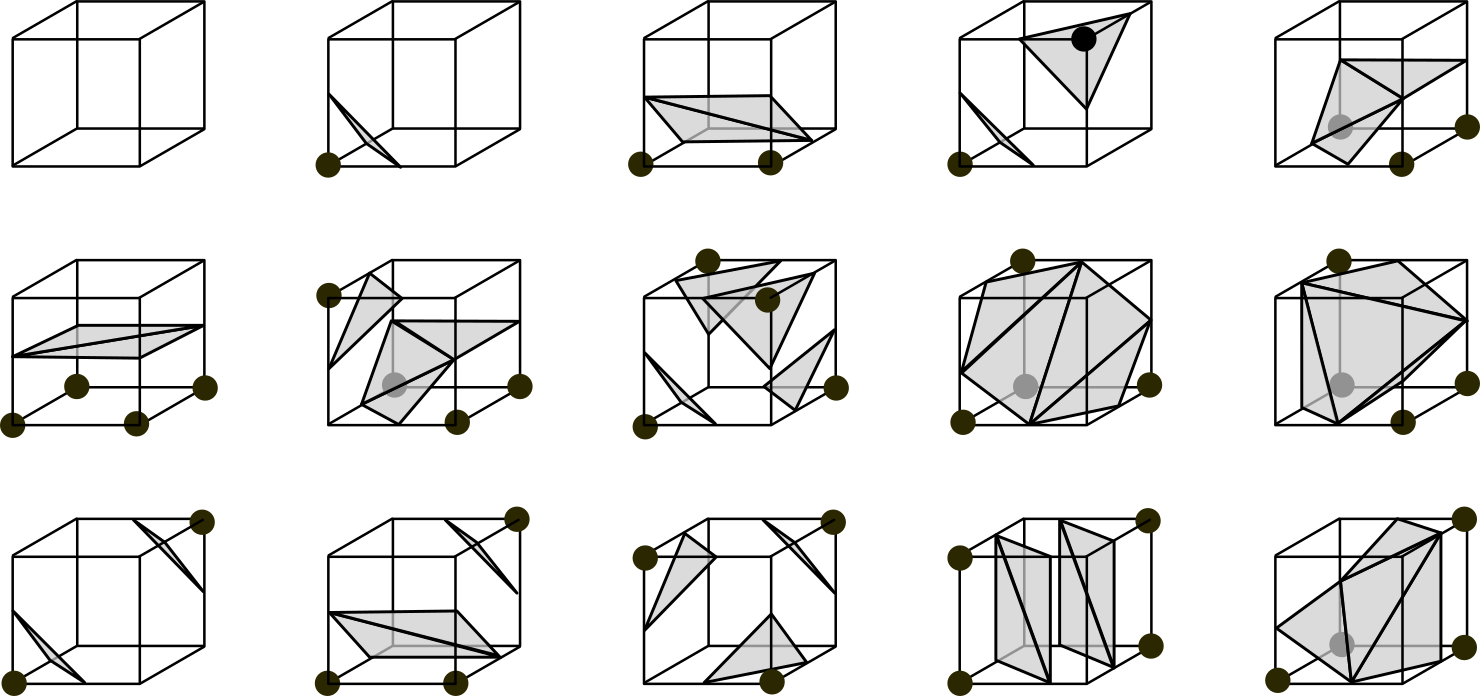
\includegraphics[width=0.95\textwidth]{images/lookup_table}}
    \caption[Zredukovaná vyhľadávacia tabuľka pre algoritmus Marching Cubes]
    {Zredukovaná vyhľadávacia tabuľka \cite{smistad2012real} pre algoritmus \textit{Marching Cubes}.}
    %id obrazku, pomocou ktoreho sa budeme na obrazok odvolavat
    \label{obr:lookup_table}
\end{figure}

Približná poloha priesečníka s hranou kocky sa dá vypočítať napríklad pomocou lineárnej interpolácie, avšak 
dajú sa použiť aj presnejšie, avšak pomalšie, interpolácie vyšších rádov. Najrýchlejšia avšak najmenej presná
možnosť je zvoliť ako priesečník stred hrany kocky.

Analógiu tejto metódy pre $2D$ môžeme vidieť na obrázku \ref{obr:marching_cubes}. V tomto prípade delíme rovinu na štvorce, 
vypočítame vrcholy nachádzajúce sa vnútri alebo na hranici. Tieto vrcholy sú na obrázku znázornené 
červenou farbou. V tomto prípade sú za priesečníky zvolené stredy hrán znázornené modrou farbou. 
Pre $2D$ prípad existuje len $2^4 = 16$ možností, avšak aj tento počet sa dá vďaka symetriám zredukovať.


\begin{figure}
    \centerline{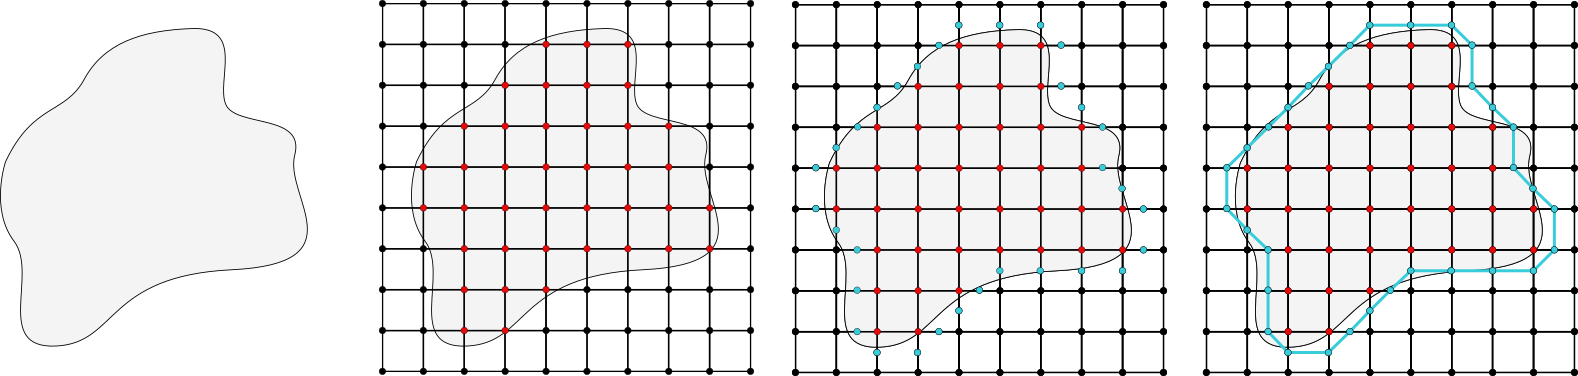
\includegraphics[width=0.95\textwidth]{images/marching_cubes}}
    \caption[Analógia metódy Marching Cubes]{Analógia metódy \textit{Marching Cubes} pre $2D$.}
    %id obrazku, pomocou ktoreho sa budeme na obrazok odvolavat
    \label{obr:marching_cubes}
\end{figure}

Táto metóda však má v niektorých prípadoch problémy s nejednoznačnosťou. Pre niektoré kombinácie
nevieme jednoznačne rozhodnúť ako by mali vyzerať výsledné trojuholníky pre danú kocku. Prípad takejto
nejednoznačnosti môžeme vidieť na obrázku \ref{obr:mc_ambiguities}. Vidíme, že v tomto prípade sú $2$ 
možné spôsoby, ktorými môžeme lokálne aproximovať hranicu oblasti. Rovnaké problémy nastávajú aj v $3D$
verzii algoritmu. Mnohí autori sa venovali riešeniu tohto problému. Najjednoduchší spôsob je navzorkovať
kocku v jej strede a rozhodnúť sa na základe výsledku, čo však nemusí vždy fungovať. O riešenie týchto 
nezrovnalostí sa pokúsili napríklad Nielsen et al.\cite{nielson1991asymptotic},
Durst et al. \cite{durst1988re}, Baker et al. \cite{baker1989building},
Cline and Lorensen \cite{cline1988two}. Táto téma je už mimo rozsah našej práce.

\begin{figure}
    \centerline{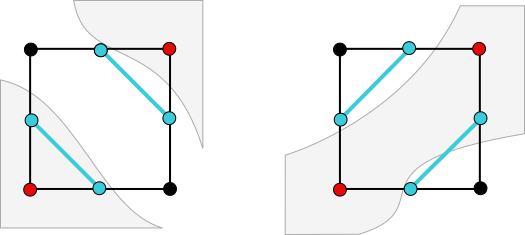
\includegraphics[width=0.6\textwidth]{images/mc_ambiguities}}
    \caption[Nejednoznačnosť Marching Cubes]{Nejednoznačnosť \textit{Marching Cubes} pre $2D$.}
    %id obrazku, pomocou ktoreho sa budeme na obrazok odvolavat
    \label{obr:mc_ambiguities}
\end{figure}



\section{Delaunayova triangulácia}
\label{kap:delaunay_triangulation}

\begin{definition}
    (difeomorfizmus)

    Pod difeomorfizmom medzi dvoma diferencovateľnými 2D varietami $\mathbf{A}$ a $\mathbf{B}$ 
    rozumieme existenciu zobrazenia $\varphi : \mathbf{A} \to \mathbf{B}$, pričom toto zobrazenie 
    je invertibilné a obe zobrazenia, $\varphi$ aj $\varphi^{-1},$ sú spojite diferencovateľné do určitého rádu. 
\end{definition}

V tejto časti sa budeme venovať lokálnej podmienke pre potenciálny trojuholník, ktorý chceme pridať do 
\textit{meshu}. Podmienka zaisťuje neprekrývajúce sa trojuholníky, a teda topologickú 
ekvivalenciu implicitne definovanej plochy a vytvoreného \textit{meshu}.

Podľa článku \textit{Marching triangles: Delaunay implicit surface triangulation} \cite{hilton1997marching} 
je \textit{3D Delaunayova triangulácia} ľubovoľnej množiny bodov $X\in \mathbb{R}^3$
zložená z takých štvorstenov, že pre každý z nich existuje guľa prechádzajúca cez každý z vrcholov 
štvorstenu, ktorá neobsahuje žiadne iné body z $X$. V prípade, že body $X$ ležia na \textit{2D variete} 
odvodil \textit{J.D.Boissonnat} \cite{boissonnat1984geometric} nasledujúcu vlastnosť. Trojuholník
lokálne difeomorfný s \textit{2D varietou} je v \textit{3D Delaunayovej triangulácii}, ak spĺňa 
\textit{Delaunayovu vlastnosť}.

\begin{definition}
    (Delaunayova vlastnosť)

    Trojuholník $\mathbf{T}$ je stenou v 3D Delaunayovej triangulácii množiny vrcholov 
    $\mathbf{X}\in \mathbb{R}^3$, ak existuje guľa prechádzajúca cez vrcholy trojuholníka 
    $\mathbf{T}$ a v tejto guli sa nenachádza žiadny ďalší vrchol z $\mathbf{X}$. 
\end{definition}

Príklad trojuholníka $T$, ktorý spĺňa \textit{Delaunayovu vlastnosť} môžeme vidieť na obrázku 
\ref{obr:delaunay_face_property}. Vo sfére prechádzajúcej cez vrcholy trojuholníka $T$ 
sa nenachádza žiadny ďalší vrchol z množiny $X$ vrcholov triangulácie.

\begin{figure}
    \centerline{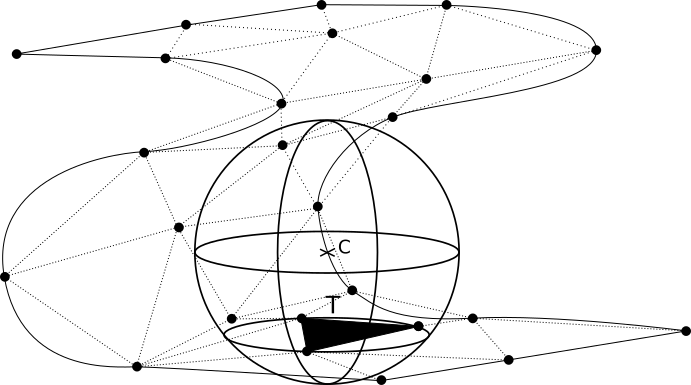
\includegraphics[width=0.6\textwidth]{images/delaunay_face_property}}
    \caption[Trojuholník $T$ spĺňajúci Delaunayovu vlastnosť]
    {\cite{hilton1996marching} Trojuholník $T$ spĺňa \textit{Delaunayovu vlastnosť}.}
    %id obrazku, pomocou ktoreho sa budeme na obrazok odvolavat
    \label{obr:delaunay_face_property}
\end{figure}

Ak túto vlastnosť spĺňajú všetky trojuholníky z mnohostenu, ktorý je \textit{difeomorfný} so zadanou
\textit{2D varietou}, tak je tento mnohosten \textit{Delaunayovou trianguláciou} uvažovanej plochy
s množinou vrcholov $\mathbf{X}$.

\textit{3D Delaunayova triangulácia} je analógiou k \textit{2D Delaunayovej triangulácii}, pričom
body z množiny $\mathbf{X}$ ležia na všeobecnejšej ploche namiesto 2D roviny.

V článku \textit{Marching triangles: Delaunay implicit surface triangulation} \cite{hilton1997marching}
autori odvodili vhodnú podmienku na pridanie trojuholníka do \textit{meshu}.

\begin{definition}
    (Delaunayova podmienka)
    \label{def:delaunay_constraint}

    Nech sa trojuholník $\mathbf{T}(x_i, x_j, x_{new})$ skladá z hraničnej hrany $\mathbf{e}(x_i, x_j)$ 
    meshu $\mathbf{M}$ a vrchola $x_{new}$. Tento trojuholník môžeme pridať do 
    $\mathbf{M}$ iba vtedy, ak sa z doterajšej 
    množiny vrcholov žiadny vrchol, ktorý je súčasťou trojuholníka s rovnakou orientáciou ako 
    $\mathbf{T}$ nenachádza vnútri gule prechádzajúcej cez vrcholy $x_i, x_j, x_{new}$ so stredom 
    v bode C, pričom C je stred opísanej kružnice trojuholníka $\mathbf{T}$.
\end{definition}

    Pod rovnakou orientáciou 
    trojuholníkov $T_1$ a $T_2$ myslíme podmienku kladného skalárneho súčinu ich normál, teda 
    $\vec{n}_1 \cdot \vec{n}_2 > 0$.

\begin{figure}
    \centerline{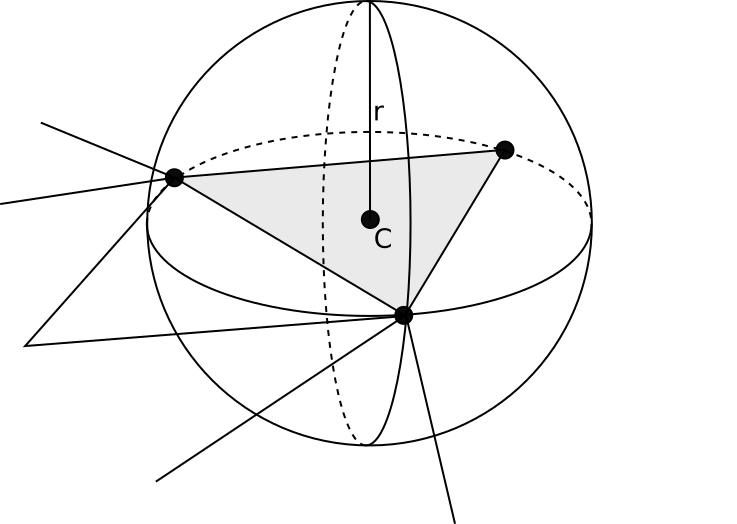
\includegraphics[width=0.6\textwidth]{images/delaunay_constraint}}
    \caption[Trojuholník $T$ spĺňajúci Delaunayovu podmienku]
    {\cite{hilton1996marching} Trojuholník $T$ spĺňa \textit{Delaunayovu podmienku}.}
    %id obrazku, pomocou ktoreho sa budeme na obrazok odvolavat
    \label{obr:delaunay_constraint}
\end{figure}

Príklad trojuholníka $T$, ktorý spĺňa \textit{Delaunayovu podmienku} môžeme vidieť na obrázku 
\ref{obr:delaunay_constraint}. V guli predchádzajúcej cez vrcholy trojuholníka $T$ so stredom 
rovnakým, ako má kružnica opísaná trojuholníku sa nenachádza žiadny vrchol z množiny vrcholov.

\textit{Delaunayova podmienka} je akási aproximácia \textit{Delaunayovej vlastnosti}. Používame ju najmä pre jednoduchšiu
implementáciu. Implementácia \textit{Delaunayovej vlastnosti} by vyžadovala
hľadanie prázdnej \textit{Delaunayovej gule}. Týchto gulí je však nekonečne veľa, keďže množina
bodov v priestore, ktoré sú v rovnakej vzdialenosti od všetkých troch vrcholov trojuholníka je priamka.
Platnosť \textit{Delaunayovej podmienky} teda zjavne zabezpečuje platnosť \textit{Delaunayovej vlastnosti}, 
no iba pre nový trojuholník.
Určenie stredu gule ako stred opísanej kružnice trojuholníku prináša veľké obmedzenie,
lebo voľný priestor v okolí plochy musí byť aspoň polomer tejto gule. Teda opačne orientovaná
časť plochy nesmie prechádzať bližšie k trojuholníku, ako je polomer gule.

Táto podmienka sa dá oslabiť druhou časťou
\textit{Delaunayovej podmienky} a to tým, že povolíme trojuholníkom s opačnou orientáciou mať vrcholy vnútri
\textit{Delaunayovej gule}. Vďaka tomuto oslabeniu dokážeme vytriangulovať aj zložitejšie plochy.


\section{Marching Triangles}

\label{kap:marching_triangles}

Algoritmus \textit{Marching Triangles} patrí do skupiny algoritmov založených na takzvanom 
sledovaní plochy. Prvý krát bol prezentovaný v roku 1996 \cite{hilton1996marching}. 
Oproti algoritmu \textit{Marching Cubes} je pomalší, avšak produkuje kvalitnejšiu trianguláciu. 

Prístupov je však viacero, v článku od autorov A. Hilton a J. Illingworth \cite{hilton1996marching}
je sledovanie plochy dosiahnuté posúvaním hrán na okraji, pričom v každom kroku sa vytvorí 
najviac $1$ trojuholník. V prístupe E. Hartmanna \cite{hartmann1998marching} sa v jednom kroku 
vytvára aj viac trojuholníkov. Algoritmus v každom kroku premieta na plochu polygón vytvorený
v hraničnom vrchole $V$ s najmenším \textit{uhlom defektu}. 

\begin{definition}
    Uhol defektu $\delta$ je definovaný ako 
    $$ \delta = 2 \pi - \sum_{i=1}^{n} \alpha_i,$$
    kde $\alpha_i$ sú uhly trojuholníkov, ktoré obsahujú vrchol $V$, pri danom vrchole $V$.
    Vizualizáciu môžeme vidieť na obrázku \ref{obr:defect_angle}.
\end{definition}


\begin{figure}
    \centerline{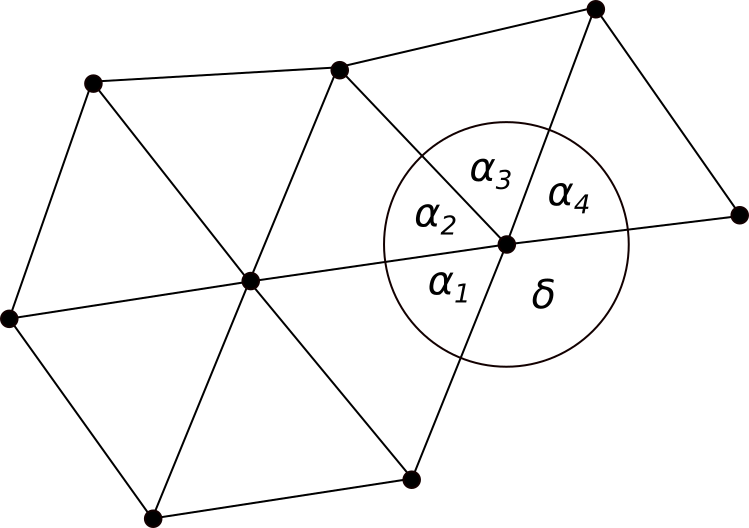
\includegraphics[width=0.4\textwidth]{images/defect_angle}}
    \caption[Uhol defektu]
    {Ilustrácia výpočtu \textit{uhla defektu} $\delta$.}
    %id obrazku, pomocou ktoreho sa budeme na obrazok odvolavat
    \label{obr:defect_angle}
\end{figure}

Postup vytvárania nových trojuholníkov môžeme vidieť na obrázku \ref{obr:Marching_triangles_by_Hartmann}.

\begin{figure}
    \centerline{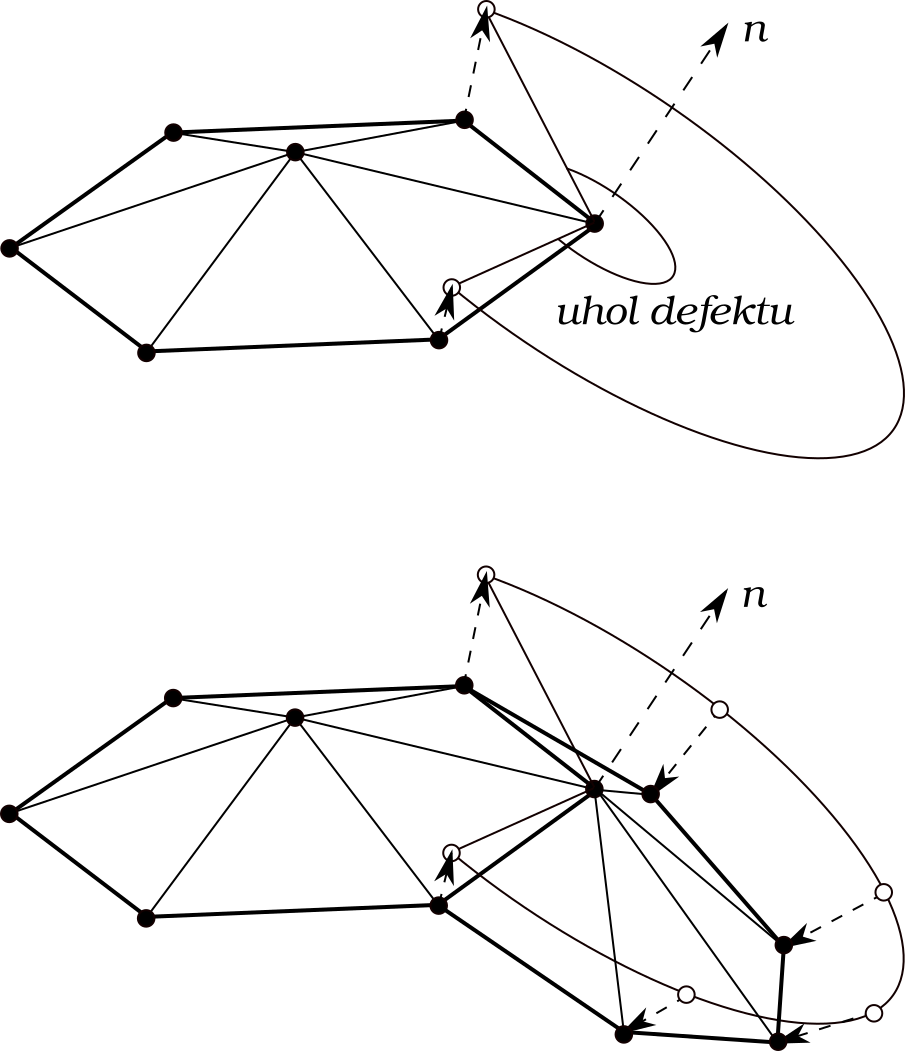
\includegraphics[width=0.45\textwidth]{images/Marching_triangles_by_Hartmann}}
    \caption[Algoritmus Marching Triangles podľa E. Hartmanna]
    {Algoritmus \textit{Marching Triangles} podľa E. Hartmanna \cite{hartmann1998marching}.}
    %id obrazku, pomocou ktoreho sa budeme na obrazok odvolavat
    \label{obr:Marching_triangles_by_Hartmann}
\end{figure}

Algoritmus od A. Hiltona et al.~\cite{hilton1996marching} začína vo vybranom bode na ploche. 
Následne vytvorí prvý trojuholník na ploche a hrany vzniknutého 
trojuholníka vloží do zoznamu hrán na okraji $\Gamma$, tieto hrany budeme nazývať hraničné. 
Opakujúc sériu krokov postupne zväčšuje trianguláciu. V každom z týchto krokov zo zoznamu $\Gamma$
vyberie jednu hranu $E$. Táto hrana susedí práve s jedným trojuholníkom. V rovine susedného 
trojuholníka vytvorí kolmicu na hranu $E$ prechádzajúcu jej stredom, 
ako na obrázku \ref{obr:new_vertex} a následne na nej bod 
$V$ v nejakej vzdialenosti $k$. 

\begin{figure}
    \centerline{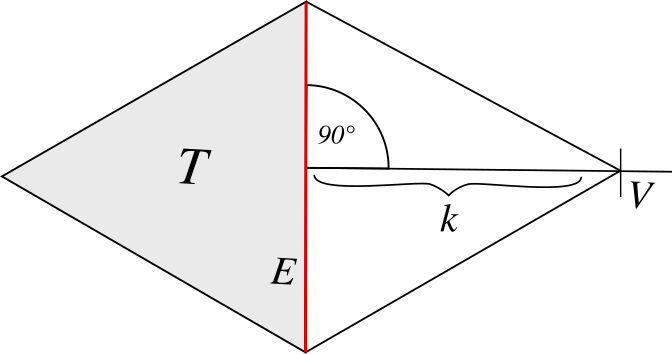
\includegraphics[width=0.45\textwidth]{images/new_vertex}}
    \caption[Vytváranie nového vrchola]
    {Vytváranie nového vrchola $V$ v rovine susedného trojuholníka $T$.}
    %id obrazku, pomocou ktoreho sa budeme na obrazok odvolavat
    \label{obr:new_vertex}
\end{figure}

Vzdialenosť $k$ môže byť daná fixne alebo môže mať premenlivú veľkosť, čím môžeme dosiahnuť 
\textit{adaptivitu na krivosť}~\cite{akkouche2001adaptive}.
V pôvodnom algoritme je táto vzdialenosť fixná. 
Následne sa tento bod pomocou numerických metód kolmo, teda v smere gradientu implicitnej funkcie, 
premietne na plochu a overí sa 
\textit{Delaunayova podmienka} pre novovzniknutý trojuholník. 
Ak trojuholník spĺňa \textit{Delaunayovu podmienku}, pridá sa do triangulácie. V opačnom prípade sa snažíme 
vytvoriť iný trojuholník skladajúci sa z pôvodnej hrany a vrcholov, ktoré sú susedné k vrcholom tejto hrany. 
V prípade, že ani tieto trojuholníky nespĺňajú \textit{Delaunayovu podmienku}, pokúsime sa vytvoriť 
trojuholník s hraničným vrcholom už existujúcej triangulácie ktorý pretína guľu z 
\textit{Delaunayovej podmienky}, ak taký existuje. Ak ju však ani tento trojuholník nesplní, 
testovanie danej hrany sa skončí.

Ak sa v danom kroku algoritmu pridá nejaký trojuholník do triangulácie, odoberieme hranu, 
s ktorou sme pracovali zo zoznamu a vložíme do nej novovytvorené hrany nachádzajúce sa na hranici.

Tento postup sa opakuje pokiaľ existujú neskontrolované hrany na hranici triangulácie.

Algoritmus vo svojej základnej podobe má viacero problémov. Ako si všimli aj autori S. Akkouche 
a E. Galin \cite{akkouche2001adaptive}, prvý a najzásadnejší problém je ten,
že algoritmus nekončí s hotovou konzistentnou trianguláciou, ale v \textit{meshi} môžu zostávať diery. Toto sa
dá vyriešiť v dodatočnom spracovaní. Ďalší, no menší problém, ktorý sme si všimli
je ten, že môžu vznikať úzke alebo malé trojuholníky, keďže algoritmus sa nesnaží spájať blízke vrcholy.

